% !TeX root = ./main.tex

\chapter{模型与算法描述}

\section{Navier-Stokes/Darcy 耦合模型}

“Navier-Stokes/Darcy 耦合模型”是一种描述普通介质和多孔介质共存的物理场景中的流体运动规律的偏微分方程模型。首先引入一个简化场景,如图\ref{fig:NS/D}所示:

\begin{figure}[H]
  \centering
  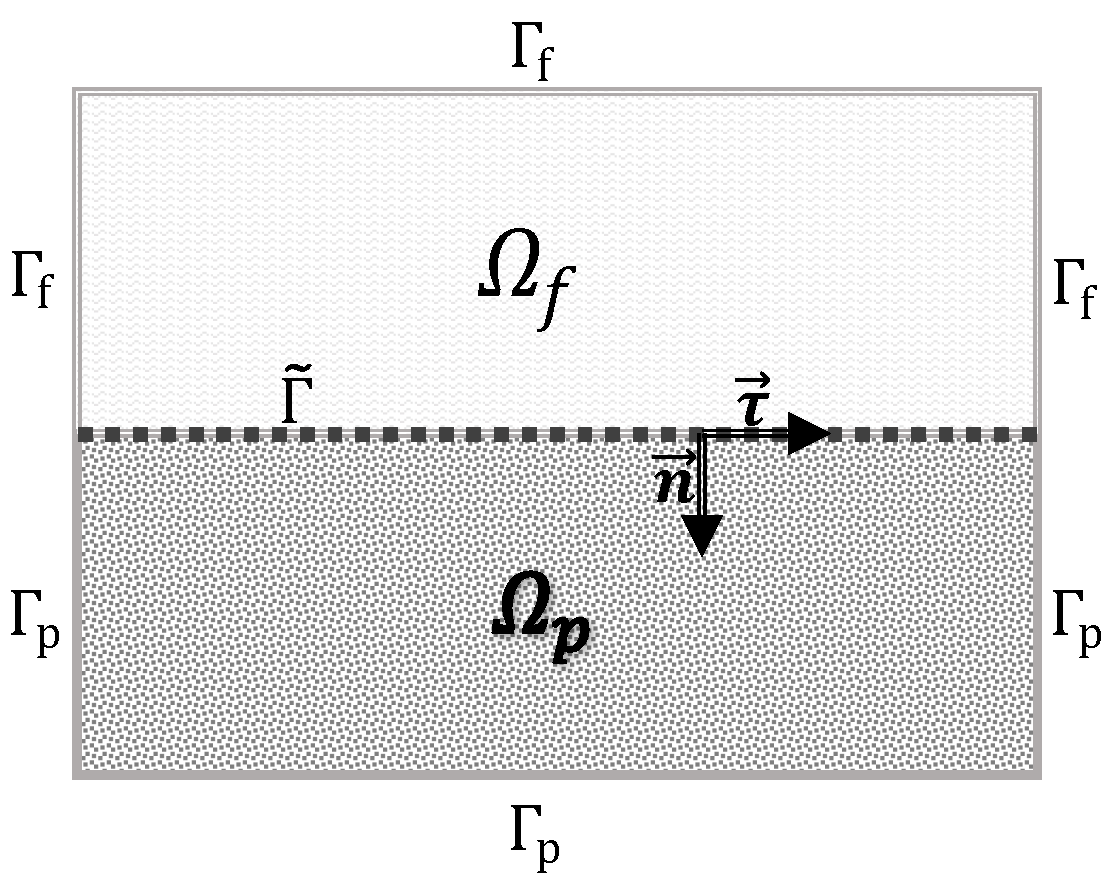
\includegraphics[width=0.5\linewidth]{images/NS-D简化示意图.pdf}
  \caption*{\small \textit{图示有界区域 $\Of \subset \R[d] $为自由流(free fluid)区域,有界区域 $\Op \subset \R[d]$为多孔介质流(porous media flow)区域, $d = 2 \text{或} 3$ 代表空间维度。$\Of \cap \Op = \emptyset$, 而两区域相邻边界 $\iB = \bar{\Of} \cap \bar{\Op}$ 称为交界面(interface)。在交界面 $\iB$ 上任意一点的单位法向量(由自由流区域 $\Of$ 指向多孔介质流区域 $\Op$)记为 $\vec n$ ;任意一点的切空间的正交基记为 $\vec \tau_i,i=1,\cdots,d-1$ (对于如图所示 $d=2$ 的情况,任意一点的切空间的正交基即为其切向量本身,记为 $\vec \tau$)。$\Of,\Op$除交界面之外的其他边界记为 $\Bf = \partial \Of / \iB,\Bp = \partial \Op / \iB$。除此之外,模型将关注一段时间范围内的流体运动,此时间范围记作 $ T = \left[ t_0,t_1 \right] \subset \R$。}}
  \caption{NS/D简化示意图}
  \label{fig:NS/D}
\end{figure}

\subsection{Navier-Stokes 方程组}

自由流区域 $\Of$ 的流体运动由 Navier-Stokes 方程组控制:

\begin{equation}\label{eq:NS}
\left\{
    \begin{aligned}
        \rho \left(\toD{\Uf}{t} + (\Uf \cdot \gradOp) \Uf \right) - \gradOp \cdot \opTf &= \rho\gf & & \textrm{ in } \Df\\  
        \gradOp \cdot \Uf &= 0 & & \text{ in } \Df
    \end{aligned}
\right.
\end{equation}

方程中符号涉及到的物理单位列出如下:
\begin{itemize}
\item $\Uf : m \cdot s^{-1}$
\item $\pf : kg \cdot m^{-1} \cdot s^{-2}$
\item $\rho : kg \cdot m^{-3}$
\item $\mu : kg \cdot m^{-1} \cdot s^{-1}$
\item $\gf : m \cdot s^{-2}$
\end{itemize}

其中:
$\rho$ 为流体密度,由于假设流体是不可压缩的,所以看做一个常量。

$ \Uf(\vec{x};t) \in \C[2](\Df; \R[d]); \vec{x} \in \Of, t \in T$ 代表流体速度场函数, $d$ 代表空间维数;$t$ 代表时间。$ \pf \in \C[1](\Df; \R) $ 代表流体的压力函数。$ \gf \in \C(\Df; \R[d])$ 代表流体受到的合外加速度场函数,实际情况下一般会取重力场。

$\opTf = 2 \mu \opDf - \pf \matfmt{I}$ 被称为柯西应力张量(Cauchy stress tensor),其中 $\mu$ 为流体动黏滞度(Dynamic viscosity), 看作一个常数参数; $\opDf = \frac{1}{2}(\gradOp \Uf + {\gradOp \Uf}^T)$ 被称为形变张量(deformation tensor),$\matfmt{I}$ 为单位矩阵。

通常该方程组还需要补充初边界条件才能进行求解,本文默认使用狄利克雷边界条件,表示如下:

\begin{equation}
\left\{\begin{aligned} 
    \Uf &= \Uf^{\Bf} & & \text{ on } \BDf,\\
    \Uf &= \Uf^{t_0} & & \text{ in } \IDf.
\end{aligned}\right.
\end{equation}

\subsection{Darcy 方程组}

多孔介质流区域 $\Op$ 中流体运动由以下方程组描述:

\begin{equation}\label{eq:Darcy}
\left\{
    \begin{aligned}
        S_0 \toD{\pp}{t}+\gradOp \cdot \Up &=\fp & & \text { in } \Dp, \\
        \Up &= -\matfmt{K} \gradOp \pp & & \text { in } \Dp.
    \end{aligned}
\right.
\end{equation}

方程中符号涉及到的物理单位列出如下:
\begin{itemize}
    \item  $S_0 : \text{ 常数 }$
    \item  $\Up : m \cdot s^{-1}$
    \item  $\fp : s^{-1}$
    
    
    \item  $\pp = z + \frac{p_p}{g\rho}: m$
    \item  $p_p : kg \cdot m^{-1} \cdot s^{-2}$
    \item  $\rho : kg \cdot m^{-3}$
    \item  $g : m \cdot s^{-2}$
    
    \item  $\matfmt{K} = \frac{\rho g \kappa \matfmt{I} }{\mu} : m \cdot s^{-1}$
    \item  $\kappa : m^2$
    \item  $\mu : kg \cdot m^{-1} \cdot s^{-1}$
\end{itemize}

其中:
$S_0$ 为质量比储存相关系数(specific mass storativity coefficient)。
$\phi = z + \frac{p_p}{g\rho}$ 称为“测压头(pressure head)”,“测压头”本来意义是液柱的高度,它能够代表液柱对容器底部的压力大小,在流体力学实验中就是与流体压力相关的一个量。这里的$p_p$就代表着多孔介质区域中流体的动态压力(dynamic pressure),或者称为 Darcy 压力,$g$ 为重力加速度,$p$ 为流体密度,$z$是一种相对深度,称为海拔标头(elevation head),可以看作一种常数参数。因此 $\phi$ 与 $p_p$ 就是一种线性关系,对方程本身来说区别不大。
$\matfmt{K} = \frac{\rho g \kappa \matfmt{I} }{\mu}$ 为导水率(Hydraulic conductivity),它代表了多孔介质中流体流动的难易程度,其中 $k$ 为渗透率(permeability),$\mu$ 为动态粘度(Dynamic viscosity)。

方程组中第二个式子即为 Darcy定律,它的物理含义基本上就是说多孔介质中流速与压力的梯度是负线性相关的,这在直观上很容易理解:压力没有变化,那流体是平静的没有运动;存在压力差,那么流体就会相应运动。本方程组同样需要补充初边值条件才能进行求解,本文也形式化地表示如下:

\begin{equation}
\left\{
    \begin{aligned}
        \pp &=\pp_{\Bp} & & \text { on } \BDp, \\
        \pp &=\pp^{t_0} & & \text { in } \IDp.
    \end{aligned}
\right.
\end{equation}

\subsection{交界面条件}

除了控制两个区域流体运动的方程组之外,本模型中还有一项重要约束就是耦合这两区域流体运动的交界面条件了,\eqref{eq:Interface} 为分别从物理学的三个角度构建的交界面条件:

\begin{equation}\label{eq:Interface}
    \begin{aligned}
        \Uf \cdot \vec{n} &= \Up \cdot \vec{n} \quad \text{ on } \iB \\
        -\left(\opTf \vec{n} \right) \cdot \vec{n} &= g \rho (\pp - z) \quad \text{ on } \iB \\
        -\left(\opTf \vec{n} \right) \cdot \vec{\tau}_i &= \alpha \sqrt{\frac{g \rho \mu}{(\matfmt{K} \vec{\tau}_i) \cdot \vec{\tau}_i}} (\Uf - \Up) \cdot \vec{\tau}_i, i=1, \cdots ,(d-1) \quad \text{ on } \iB \\
    \end{aligned}
\end{equation}

其中第一个公式代表了交界面的质量守恒定律,直观含义即为两区域在交界面法线方向的流速相等;第二个公式为交界面的压力平衡条件;第三个公式被称为 Beavers-Joseph 交界面条件 \cite{beavers1967boundary}(简称BJ条件),其中 $\alpha$ 在实践中是一个需要通过实验确定的常数参数。这三个交界面条件共同约束着本模型中两区域流体运动进行着的相互作用。

以上公式涉及到的一些符号约定如下:

$\gradOp = (\toD{}{x_1},\cdots,\toD{}{x_d})^T$ 为空间梯度算子(只对空间维度求梯度)。

$\Uf \cdot \gradOp = \sum_{i=1}^{d} \Ufi \cdot \toD{}{x_i} $ ,其中 $x_i$ 表示空间维度第i个分量, $\Ufi \in \C[2](\Df; \R)$ 为对应分量的速度大小(函数),也就是说,$\Uf = \overrightarrow{\left(\Ufi[1],\cdots,\Ufi[d]\right)}$。

$ \laplaceOp = \gradOp^2 = \gradOp \cdot \gradOp = \sum_{i=1}^{d} \toDsqua{}{x_i}$ 为空间拉普拉斯算子。

当算子与函数由“$\cdot$”连接时代表以向量点积的形式作用,如 $\gradOp \cdot \Uf = \sum_{i=1}^{d} \toD{\Ufi}{x_i}$等,所以“$\gradOp \cdot$”本质上代表的是散度算子;当算子直接连接函数且函数为向量函数时,则代表数乘或矩阵作用,如 $ \laplaceOp \Uf = (\sum_{i=1}^{d} \toDsqua{\Ufi[1]}{x_i},\cdots,\sum_{i=1}^{d} \toDsqua{\Ufi[d]}{x_i})_{1 \times d}; \gradOp \Uf = \left(a_{i j} = \toD{\Ufi[j]}{x_i} \right )_{d \times d}$ 。

\section{神经网络与深度学习算法}

神经网络是深度学习中一种函数拟合的工具,它可以拟合各种所需要的未知函数。

\subsection{神经网络模型}

神经网络模型最初是受到大脑中神经元结构的启发建立的。神经元有三个特点,1.它具有多个输入,一个输出;2.神经元的输入通过突触传递,其粗细不一,意味着传递信号的能力不同;3.输入可以叠加,但是输出有一定范围且存在阈值,也就是说输出与输入并不是线性关系。

首先建立单个神经元的数学模型:根据特点1,把神经元看作一个定义在向量空间中的实值函数 $ e(\vec{x}):\R[n] \longmapsto \R $,其中 $\vec{x} = (x_1, \cdots, x_n)$ 作为n维向量代表神经元有n个输入;根据特点2,定义权重向量 $\vec{w} = (w_1,\cdots, w_n) \in \R[n]$,其中 $w_i$ 代表输入 $x_i$ 对应的信号权重;再跟据特点3,引入一个有界非线性函数(后面称其为激活函数) $\sigma:\R \longmapsto \R$ 以及一个阈值参数(后面称其为偏置) $b \in \R$,最后得到单个神经元的数学模型表示为公式 ~\eqref{eq:e}:

\begin{equation}\label{eq:e}
    e(\vec{x}) = \sigma(\vec{w} \cdot \vec{x} + b)
\end{equation}

下面定义单层全连接神经网络模型,它是由共享同一个输入的多个神经元组合而成,设输入为 $\vec{x} \in \R[n]$,且被 $m$ 个神经元 $e_i(\vec{x}) = y_i,i=1,\cdots,m$ 共享,那么整个单层神经网络模型可以看作一个 $m$ 维向量值函数 $\vec{l}(\vec{x}) = (e_1(\vec{x}), \cdots, e_m(\vec{x})):\R[n] \longmapsto \R[m]$,同时一般规定一层神经网络中所有神经元的激活函数 $\sigma_i$ 都相同,记作 $\sigma_i = \sigma, i=1, \cdots, m$, 所以最终单层模型表示为公式 ~\eqref{eq:l} 

\begin{equation}\label{eq:l}
    \vec{l}(\vec{x}) = \sigma(\vec{x}\matfmt{W} + \vec{b})
\end{equation}

其中权重矩阵为: 

\newcommand{\Wmat}{
    \begin{pmatrix}  
        w_{1 1} & \cdots & w_{1 m} \\  
        \vdots & \ddots & \vdots \\  
        w_{n 1} & \cdots & w_{n m}  
    \end{pmatrix}
}

\begin{equation*}
    \matfmt{W} = \Wmat \in \R[n \times m]
\end{equation*}

$w_{i j}$ 为第 j 个神经元函数中权重向量的第 i 个分量。

偏置向量 $\vec{b}=(b_1, \cdots, b_m) \in \R[m]$,$b_i$ 为 $e_i$ 的偏置,还要注意此写法中激活函数 $\sigma$ 作用在向量上指的是其直接作用在向量的每一个分量上。

最经典的全连接神经网络(Fully Connected Neural Network)模型就是由多个单层全连接网络模型进行叠加而组成的,$s$ 层全连接网络可表达为
\newcommand{\NNF}[1][\cdot]{\NN(#1,\params)}

\begin{equation}
    \begin{aligned}
        \NNF[\vec{x}] &= \left( \vec{l_s} \circ \cdots \circ \vec{l_1}\right)(\vec{x}) \\ 
        &= \sigma_s(\cdots\sigma_2(\sigma_1(\vec{x}\matfmt{W}_1 + \vec{b}_1) \matfmt{W}_2 + \vec{b}_2)\cdots\matfmt{W}_s + \vec{b}_s)
    \end{aligned}
\end{equation}

其中 $\circ$ 为函数复合运算, $\vec{l}_i(\vec{x}_i),i=1, \cdots, s$ 为单层全连接网络, $\matfmt{W}_i, \vec{b}_i$ 为 $\vec{l}_i(\vec{x}_i)$ 的权重矩阵和偏置向量;不同的 $\vec{l}_i(\vec{x}_i)$ 的权重和偏置可以不同,输入与输出维度也可能不同,但是要求 $\vec{l}_i(\vec{x}_i)$ 的输出维度与 $\vec{l}_{i+1}(\vec{x}_{i+1})$ 的输入维度相同,这样才能进行函数复合,也就是说,设 $n_k$ 为 第 $k$ 层网络的输入维度,则 $\matfmt{W}_k \in \R[n_k \times n_{k+1}],b_{k} \in \R[n_{k+1}], k=1,\cdots,s-1$ ;集合 $\params =  \{w_{ij;k}, b_{i;k} \mid \matfmt{W}_k = (w_{ij;k}), \vec{b}_k = (\cdots, b_{i;k},\cdots), k=1,\cdots,s \}$ 统称为该神经网络的参数,对于相同的输入参数发生改变则神经网络的输出也就发生了改变;易得 $\params \in \paramset := \R[\sum_{k=1}^{s-1} n_k \times n_{k+1} + n_{k+1}]$。因此,一个全连接神经网络可以看作就是具有上述公式结构的拥有参数 $\params$ 的向量值函数。值得注意的是,在实践中神经网络的激活函数一般都为连续函数或者满足 $\sigma \in L^p (\R; \R) $,因此这里不妨假设 $\NNF \in L^p(\R[n]; \R[m]),1 \le p < \infty.$,同时最后一层的激活函数往往不设置或着看作规定为恒等函数:$\sigma_s (x) = x$,这样做以避免神经网络只能输出有限范围的值。

\subsection{损失函数}\label{sec:Loss}

神经网络模型的结构及其大量的参数使得其拥有一种强大的函数拟合能力。所谓其函数拟合能力,首先要定义一种衡量神经网络 $\NNF$ 与待拟合函数 $\vec{f}$ 的“距离”的标准;假设 $\vec{f}, \NNF \in L^p(\R[n]; \R[m])$,最自然的方式就是使用函数空间 $L^p$ 的范数进行构造:

\begin{equation}
    \begin{aligned}
        d(\NNF,\vec{f}) = \| \NNF-\vec{f} \|_{\Lp} = \left( \int_{X} \left\| \NNF-\vec{f} \right\|^{p}_{l^{p}} \mathrm{d}\vec{x} \right)^{\frac{1}{p}}
    \end{aligned}
\end{equation}

其中 $X \subseteq \R[n]$ 为 $\vec{f}(\vec{x})$ 的定义域,这里假设 $X$ 是有界的;$\| \cdot \|_{l^{p}}$ 是向量值域空间 $\R[m]$ 的p范数。对于函数 $\vec{f}(\vec{x})$ 以及一个预先指定的极小量 $0 < \varepsilon \ll 1$(如 $1^{-10}$),若存在一个神经网络 $\NNF$,使得 $d(\NNF,\vec{f}) < \varepsilon$,则称该神经网络 $\NNF$ 拥有对函数 $\vec{f}(\vec{x})$ 的拟合能力。

事实上大名鼎鼎的通用近似定理(Universal approximation theorem,其实它不是具体某一个定理,而是代表历史上对神经网络拟合能力的刻画越来越强的一组定理)\cite{hornik1991approximation,hornik1989multilayer,hornik1990universal} 指出,在满足一定的条件下的神经网络对给定的函数空间内(如 $\Lp$ 空间)的任意函数均拥有很强的拟合能力,关于它的细节将在第三章中描述。

然而在实践中所关心的是如何找到一个成功拟合了所需函数的神经网络。标准做法是,对于待拟合函数 $\vec{f}$ ,先通过经验确定一个神经网络的结构 $\NNF$,结构就是指其网络层数,每层的激活函数以及权重矩阵和偏置向量的形状,但是具体的参数值待定。随后将问题转化为对该神经网络参数的优化问题 ~\eqref{eq:Optimize}:

\begin{equation} \label{eq:Optimize}
    \begin{aligned}
        \min_{\params \in \paramset} \| \NNF- \vec{f}\|_{\Lp}.
    \end{aligned}
\end{equation}

接下来的目标就是使用各种优化算法对该问题进行求解,这个过程通常被称为“神经网络的训练”。

但是在实践中,计算机无法处理无限多个数据,因此不能直接对上述优化问题中的积分进行计算,而是使用了一种数值积分的算法进行逼近:首先对定义域 $X$ 进行均匀随机采样,得到一个有限集合 $\hat{X}  \subset X \subseteq \R[n]$ ,然后令 $\toTset{\hat{X}} = \{\x,\vec{f}(\x) \mid \x \in \hat{X}\}$, 通常称集合 $\toTset{\hat{X}}$ 为“训练集”;另一方面,在大多数问题中待拟合函数 $\vec{f}$ 本就是未知的,只能采样到其部分输入输出作为训练集,此时也往往假设采样到的分布为均匀随机的。随后计算 $\frac{\toInt{X}{1}{x}}{|\hat{X}|}\sum_{\x,\vec{f}(\x) \in \toTset{\hat{X}}} \sum_{i=1}^{m} \left| \NNF_{\x_i} - \vec{f}_{x_i}(\x) \right|^{p}$ 作为对积分 $\toInt{X}{\left\| \NNF-\vec{f}(\vec{x}) \right\|_{l_p}^{p}}{\vec{x}}$ 的数值估计;在均匀随机采样的假设下可以看出估计的期望即为原积分的值。此时原优化问题变为如下 ~\eqref{eq:EstiOptm} 形式:

\begin{equation}\label{eq:EstiOptm}
    \min_{\params \in \paramset} \left(\frac{\toInt{X}{1}{x}}{|\hat{X}|}\sum_{\x,\vec{f}(\x) \in \toTset{\hat{X}}} \sum_{i=1}^{m} \left| \NNF_{\x_i} - \vec{f}_{x_i}(\x) \right|^{p} \right)^{\frac{1}{p}}.
\end{equation}

作为目标函数,不妨假设 $\toInt{X}{1}{x} = 1$,记 $N_{\toTset{\hat{X}}} = |\toTset{\hat{X}}| = |\hat{X}|$ ,同时去掉最外层的 $(\cdot)^{\frac{1}{p}}$ 以简化计算量。此时 该问题的目标函数变为 ~\eqref{eq:Target}:

\begin{equation}\label{eq:Target}
    \LossX = \toLoss{\hat{X}}{\x,\vec{f}(\x)}{m}{\NNF_{\x_i} - \vec{f}_{x_i}(\x)}
\end{equation}

该目标函数在神经网络的训练中被称为损失函数。

针对不同的问题,也有很多其他的衡量神经网络与待拟合函数间距离的方式,其对应的损失函数的形式也会有不同。确定了损失函数以后接下来就是对神经网络进行训练了。

\subsection{神经网络的训练算法}

神经网络训练算法的目的是得到优化问题 ~\eqref{eq:Optimize} 的近似解 $\params^* = \arg \min_{\params \in \paramset} \LossX$,虽然最优化理论提供了众多优化问题的求解算法,但是对于上述神经网络的训练问题,其训练集中样本的数量往往非常大,同时神经网络的参数量也不小,因此大部分涉及到二阶微分或者线搜索的优化算法在该问题上将会产生较大的计算开销。因此目前常用的求解算法来源于相对基础的梯度下降法,同时为了进一步减少计算开销,提出了算法\ref{algo:mgd}:小批量随机梯度下降法(minibatch gradient descent)来进行神经网络的训练,具体表示如下:

\begin{algorithm}[htb]
  \caption{小批量随机梯度下降法(minibatch gradient descent)}
  \label{algo:mgd}
  \small
  \SetAlgoLined
  \KwIn{训练集 $\TX$, 神经网络 $\NNF$ 的结构,学习率 $lr$(一般取0.01),容许误差 $0 < \varepsilon \ll 1$,训练阈值参数 $n_T$, 学习率调整误差阈值 $0 < \epsilon_{lr} \ll 1$,学习率调整耐心阈值 $n_{lr}$,学习率调整衰减率 $ r_{lr} $(一般取 0.5)}
  \KwOut{ $\hat{\params}^*$ 的近似解 $\params_k$ }

  对参数 $\params$ 进行初始化,如常值初始化,Xavier 初始化 \cite{glorot2010understanding}、Kaiming 初始化 \cite{he2015delving} 等,记为 $\params_0$;令 $k = 0$\;
   \While{ $\| \mathbf{g_k} \| \le \varepsilon$ 不成立 }{
      \While{ $\TX$ 还未被全部采样过一遍或者此循环次数 $\le n_T$ }{
        从训练集中按一定规则进行一次小批量采样得到 $\hat{\mathcal{T}}_{{\hat{X}}_k} \subset \TX$。可以采用顺序采样,随机采样等方法;每次采样的样本数量取决于计算机的硬件能力\;
        将 $\params_k$ 代入基于 $\hat{\mathcal{T}}_{{\hat{X}}_k}$ 的损失函数 $L(\params_k;\hat{\mathcal{T}}_{{\hat{X}}_k})$ 中并计算其输出关于 $\params_k$ 的梯度值 $\mathbf{g_k} = \nabla_\params L(\params_k;\hat{\mathcal{T}}_{{\hat{X}}_k})$\;
        令 $\params_{k+1} = \params_k - lr \cdot \mathbf{g_k}$;
      }
      (学习率自适应调整策略:)
      \If{ 损失函数 $L(\params_k;\hat{\mathcal{T}}_{{\hat{X}}_k})$ 的值下降幅度 $< \epsilon_{lr}$的次数 $> n_{lr}$}{
          $lr = lr \times r_{lr}$
      }
  }
\end{algorithm}

目前在上述算法的基础上又衍生出一批效果更好的训练算法,如 $\textrm{Rmsprop}$ 算法, $\textrm{Adam}$ 优化器等,这些算法主要是对上述算法 \ref{algo:mgd} 中参数 $\params_k$ 的更新策略进行修改,比如考虑进多个历史梯度数据等,算法的其他部分不变,这里不再赘述。

% \subsection{训练误差与泛化误差}

% 注意到神经网络的训练在大多数情况下是一个非凸优化问题,同时其优化算法本身的结果 $\hat{\params}^*$ 也是一种近似解,更不能保证优化后的损失函数 $\Loss{}{\hat{\params}^*}{\TX} = 0$,因此这里引入训练误差的概念:

% \begin{equation}\begin{aligned}
%     \mathfrak{E}_{\TX} = L(\hat{\params}^*;\TX)
% \end{aligned}\end{equation}
% 另一方面,损失函数的结构来源于对 $L^p$ 范数的数值近似,同时训练集本身也是对待拟合函数的一次采样,因此训练后的神经网络与待拟合函数之间的客观差距不会小于训练误差,由此引入泛化误差的概念来刻画这种客观差距:

% \begin{equation}\begin{aligned}
%     \mathfrak{E}_G = d(\NN[\hat{\params}^*]{}{\cdot},\vec{f}) = \| \NN[\hat{\params}^*]{}{\cdot}-\vec{f}\|_{L^p}
% \end{aligned}\end{equation}

\section{Navier-Stokes/Darcy 耦合模型的神经网络求解方法}

本节将介绍求解上述 Navier-Stokes/Darcy 耦合 模型的双通道神经网络求解方法。求解的主要思想就是使用神经网络来拟合模型中偏微分方程的各个未知函数。针对模型的双区域结构,本文相应提出了双通道的神经网络结构,同时针对模型的方程形式提出相应的损失函数与求解算法。

\subsection{网络结构}
\newcommand{\NNFf}{\NN_f(\cdot,\params_f)}
\newcommand{\NNFp}{\NN_p(\cdot,\params_p)}
如图\ref{fig:network} 所示,整个结构由两个全连接神经网络组成:$\NNFf, \NNFp$,分别对应拟合 Navier-Stokes/Darcy 模型中的自由流区域方程组与多孔介质流区域方程组中的未知函数;其中 Navier-Stokes 方程组中包含未知函数 $\Uf,\pf$, 需要将它们的值域合并得到函数 $\vec{F}_f = ( \Ufi[1],\cdots,\Ufi[d],\pf)$ 作为网络 $\NNFf$ 的待拟合函数,同理令 $\vec{F}_p = (\Upi[1],\cdots,\Upi[d],\pp)$ 作为 $\NNFp$ 的待拟合函数。因此 $\NNFf$ 的网络输入和输出层神经元个数均为 $d+1$,至于其隐藏层的具体设置(层数,激活函数,神经元个数等)在第三章数值实验中将分别说明。

\begin{figure}[H]
  \centering
  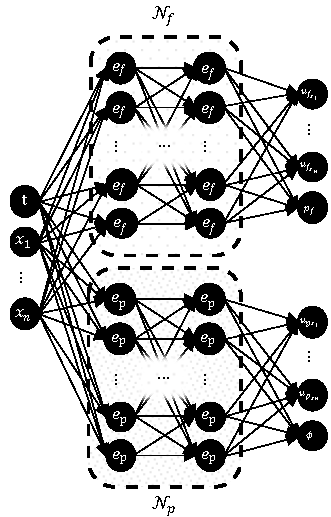
\includegraphics[width=0.5\linewidth]{images/网络结构1.pdf}
  \caption*{}
  \caption{网络结构示意图}
  \label{fig:network}
\end{figure}

\subsection{损失函数}

流体力学模型求解问题的已知条件中,关于待求解函数 $\Uf,\pf,\Up,\pp$ 本身的输入输出数据只有初边值条件,无法对全时空定义域进行均匀随机采样,因此无法完全使用传统神经网络损失函数的构造方法;另一方面,偏微分物理方程本身的约束是求解的重要条件,因此这里需要将物理方程编码进损失函数参与到神经网络的优化中去,做法如下:

设有抽象形式的物理方程 $\mathcal{P}(\vec{u}) = \vec{f} \textrm{ in } \Omega$,其中 $\mathcal{P}$ 是抽象的偏微分算子,$\vec{u} \in \Wkp{k}(\Omega; \R[m])$ 代表待解函数,$\vec{f} \in \Lp( \Omega; \R[m])$ 代表源项,$ \Omega \in \R[n]$ 为方程定义区域。

这里 $\Wkp{k}(\Omega; \R[m]) = \left\{ \vec{u} \in \Lp(\Omega;\R[m]) \mid D^\alpha(\vec{u}) \in \Lp(\Omega;\R), 0 \le |\alpha| < \infty \right\}$ 为 Sobolev 空间,其中 $\alpha = (\alpha_1,\cdots,\alpha_n); \alpha_i \in \N[+] \cup \{0\},i=1,\cdots,n$ 叫做多重指标(Multi-Index),$|\alpha| = \sum_{\alpha_i \in \alpha} \alpha_i$,$D^\alpha = \frac{\partial^{\alpha_1\cdots\alpha_n}}{\partial x_1^{\alpha_1}\cdots\partial x_n^{\alpha_n}}$ 为相应的弱导数意义下的偏微分算子。

对应设有以 $\vec{u}$ 作为待拟合函数的神经网络 $\NN_{\vec{u}}(\cdot,\params)$, 与 2.2.2 类似,定义距离函数 $\mathcal{D}(\mathcal{P},\vec{f},\NN_{\vec{u}}(\cdot,\params))) = \| \mathcal{P}(\NN_{\vec{u}}(\cdot,\params) - \vec{f} \|_{L^p(\Omega; \R[m])})$,只不过这里的距离衡量的是神经网络对物理方程的满足程度。同样需要进一步地利用数值估计将距离函数进行转换,具体的转换方法与 \ref{sec:Loss} 节所述相同,最后得到编码了物理方程的损失函数:

\begin{equation}\begin{aligned}
\LossO = \toLoss{\Omega}{\x,\vec{f}(\x)}{m}{
    \mathcal{P}(\NN_{\vec{u}}(\cdot,\params)))_{x_i}(\x)-{f}_{x_i}(\x)
}
\end{aligned}\end{equation}

根据上述的抽象做法,接下来针对本文耦合模型中各个物理方程来构造相应的损失函数。对于 $\NNFf, \NNFp$ ,首先将它们对应物理方程中待解函数的部分记为:

\begin{equation}\label{eq:NNsplit}
    \begin{aligned}
        ( \NUfi[1], \cdots, \NUfi[d], \Npf) &= (\NUf;\Npf) = \NNFf \\
        ( \NUpi[1], \cdots, \NUpi[d], \Npp) &= (\NUp;\Npp) = \NNFp
    \end{aligned}
\end{equation}

也就是说,一个多维输出神经网络也可以看作多个单输出网络的组合,只是这些网络是共享参数的。这样可以将拆分形式的 ~\eqref{eq:NNsplit} 自然代入原物理方程约束中作为拟合约束的一部分,Navier-Stokes/Darcy 模型有三部分方程约束,分别按上述方法进行损失函数的构造可得:

\begin{equation}\label{eq:Lossf}
\begin{aligned}
    \Lossf
    =& \toscaLossPre{\TDf}{\x,\gf(\x)}
    \sum_{i=1}^{d}
    \bigl\vert
        \rho \left(
                \toD{\NUfi}{t} + (\NUf \cdot \gradOp) \NUfi 
            \right) \\
    & \hspace*{10em} - \compx{(\gradOp \cdot \opT{\NUf}{\Npf{\cdot}})} - \rho \compx{\gf}
    \bigr\vert^{p} \\
    &+
    \toscaLoss{\TDf}{\x}{
        (\gradOp \cdot \NUf)(\x) - 0
    } \\
    &+
    \toLoss{\TBDf}{\x,\Uf^{\Bf}(\x)}{d}{
        \NUfi(\x) - u^{\Bf}_{f_{x_i}}
    } \\
    &+
    \toLoss{\TIDf}{\x,\Uf^{t_0}(\x)}{d}{
        \NUfi(\x) - u^{t_0}_{f_{x_i}}
    } 
\end{aligned}
\end{equation}
\begin{equation}\label{eq:Lossp}
\begin{aligned}
    \Lossp
    =& \toscaLoss{\TDp}{\x,\fp(\x)}{
        S_{0}\toD{\Npp(\x)}{t} + (\gradOp \cdot \NUp)(\x) - \fp(\x)
    } \\
    &+
    \toLoss{\TDp}{\x}{d}{
        \NUpi(\x) + \compx{(\matfmt{K} \gradOp \Npp)}
    } \\
    &+
    \toscaLoss{\TBDp}{\x,{\pp_{\Bp}}(\x)}{
        \Npp(\x) - \pp_{\Bp}(\x)
    } \\
    &+
    \toscaLoss{\TIDp}{\x,\pp^{t_0}(\x)}{
        \Npp(\x) - \pp^{t_0}(\x)
    }
\end{aligned}
\end{equation}
\begin{equation}\label{eq:Lossi}
\begin{aligned}
    &\Lossi \\
    =& \toscaLoss{\TiBD}{\x}{
        (\NUf \cdot \vec{n})(\x) - (\NUp \cdot \vec{n})(\x)
    } \\
    &+
    \toscaLoss{\TiBD}{\x}{
        -(\left(\opT{\NUf}{\Npf} \vec{n} \right) \cdot \vec{n})(\x) - g \rho (\Npp(\x) - z)
    } \\
    &+
    \sum_{i=1}^{d-1} \toscaLoss{\TiBD}{\x}{
        -(\left(\opT{\NUf}{\Npf} \vec{n} \right) \cdot \vec{\tau}_i)(\x) - \alpha \sqrt{\frac{g \rho \mu}{(\matfmt{K} \vec{\tau}_i) \cdot \vec{\tau}_i}} ((\NUf - \NUp) \cdot \vec{\tau}_i)(\x)
    }
\end{aligned} 
\end{equation}

上述构造函数 ~\eqref{eq:Lossf} ~\eqref{eq:Lossp} ~\eqref{eq:Lossi} 之和即为最终构造的损失函数 ~\eqref{eq:Lossall} :

\begin{equation}\label{eq:Lossall}
    \begin{aligned}
        &\Lossall \\
        =& \Lossf + \Lossp \\
        &+ \Lossi
    \end{aligned}
\end{equation}

\subsection{求解算法}

可以看出交界面条件所对应的损失函数同时受到两个通道神经网络参数的共同影响,这就使得训练算法能够使两神经网络进行共同训练。基于上述网络模型与损失函数的构造,结合神经网络的训练算法 \ref{algo:mgd} ,本文给出算法 \ref{algo:main} ——耦合物理信息的神经网络(Coupled-Physics-informed neural networks, cPINNs)求解算法:

\begin{algorithm}[H]
  \caption{cPINNs 算法}
  \label{algo:main}
  \small
  \SetAlgoLined
  \KwIn{耦合模型区域 $\Omega_{f} \times T, \Bf \times T, \Of \times \{t_0\}, \Omega_{p} \times T, \Bp \times T, \Op \times \{t_0\}, \iB$ 及其对应的源项函数信息, 双通道神经网络模型 $\NNFf,\NNFp$ 的隐藏层具体结构,学习率 $lr$(一般取0.01),容许误差 $0 < \varepsilon \ll 1$,Adam 优化算法参数}
  \KwOut{ ${\params_f}_{k},{\params_p}_{k}$ }

  分别对耦合模型区域 $\Omega_{f} \times T, \Bf \times T, \Of \times \{t_0\}, \Omega_{p} \times T, \Bp \times T, \Op \times \{t_0\}, \iB$ 及其对应的源项函数进行均匀随机采样,得到训练集 $\mathcal{T}_{\Omega_{f} \times T}, \mathcal{T}_{\Bf \times T},\mathcal{T}_{\Of \times \{t_0\}},\mathcal{T}_{\Omega_{p} \times T},\mathcal{T}_{\Bp \times T},\mathcal{T}_{\Op \times \{t_0\}},\mathcal{T}_{\iB}$\;
  
    对参数进行随机初始化,得到 ${\params_f}_0,{\params_p}_0$;令 $k = 0$;
    
   \While{ $\| \mathbf{g_k} \| \le \varepsilon$ 不成立 }{
      \While{ 所有的训练集还未被全部采样过一遍 }{
        对各区域训练集按数据量等比例进行随机采样,得到 $\hat{\mathcal{T}}_{\Omega_{f} \times T}, \hat{\mathcal{T}}_{\Bf \times T}, \hat{\mathcal{T}}_{\Of \times \{t_0\}}, \hat{\mathcal{T}}_{\Omega_{p} \times T}, \hat{\mathcal{T}}_{\Bp \times T}, \hat{\mathcal{T}}_{\Op \times \{t_0\}}, \hat{\mathcal{T}}_{\iB}$\;
        
        将参数代入基于第三步采样训练集的损失函数 $\mathcal{L}({\params_f}_k,{\params_p}_k;\hat{\mathcal{T}}_{\Omega_{f} \times T},\cdots,\hat{\mathcal{T}}_{\iB})$ 中并计算其输出关于 $\params_f,\params_p$ 的梯度值 $(\mathbf{g_{f_k}},\mathbf{g_{p_k}}) = \nabla_\params \nabla_\params \Loss{total}{\params_f,\params_p}{\TDf,\cdots ,\TiBD}$\;
        令 $\params_{k+1} = \params_k - lr \cdot \mathbf{g_k}$;
        
        使用Adam优化算法,令 ${\params_f}_{k+1},{\params_p}_{k+1} = \mathrm{Adam}({\params_f}_{k},{\params_p}_{k};\mathbf{g_{f_k}},\mathbf{g_{p_k}})$\;
      }
  }
\end{algorithm}

上述算法流程如图 \ref{fig:cPINNs} 所示。

\begin{figure}[t]
    \centering
    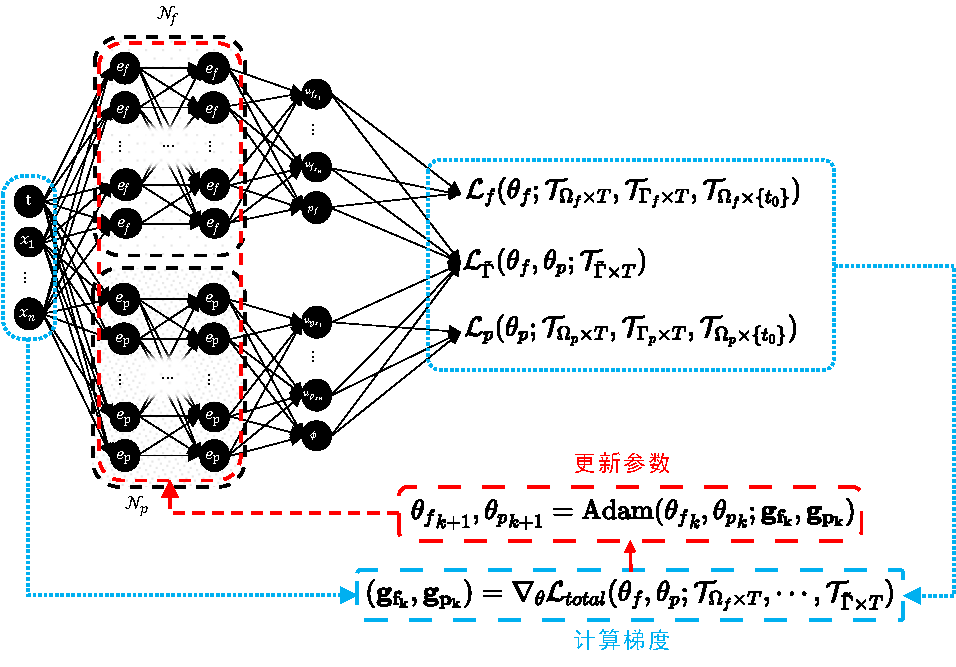
\includegraphics[width=1.0\linewidth]{images/算法2图示.pdf}
    % \caption*{}
    \caption{ cPINNs 算法流程图示 }
    \label{fig:cPINNs}
\end{figure}

\section{损失函数的合理性证明}

与众多传统算法不同,神经网络模型最初是由于实验效果的突出而得到进一步的发展与研究的,并且近些年才应用在解偏微分方程领域上,而并非由理论推导而来,因此其可解释性一直是业界关注的要点。

上述求解算法的损失函数构造基于对真解的物理方程约束的逼近,而非直接与真解距离的刻画。利用万能表示定理虽然能直接说明网络对真解的拟合能力,但还是需要特别指出网络拟合物理方程本身的能力合理性,即存在上述并行结构的全连接神经网络

\newcommand{\NNset}{\mathfrak{N}}
定理的证明主要使用文献 \cite{hornik1991approximation} 中定理3(及其讨论章节中的推论)的结果,这里重述如下:

\begin{theorem}\label{thm:approximation}
令 $\NNset = \bigl\{\NN_{one}(\vec{x},\params) = \vec{w}_2 \cdot \sigma_1(\vec{x}\matfmt{W_1} + \vec{b}_1) \mid \matfmt{W_1} \in \R[n \times m]; \vec{b}_1,\vec{w}_2 \in \R[m]; m \in \N[+] \bigr\}$,该集合为全体具有一层隐藏层且单个输出的全连接网络,其激活函数 $\sigma_1$ 为作用在每个分量上的非常值有界函数,若 $\sigma_1 \in \C[k](\R;\R)$ 是至少 k 次连续可微的, $\Omega \in \R[n]$ 为有界区域且满足一种分段条件(The Segment Condition)\cite{adams2003sobolev},则集合 $\NNset$ 在 $\Wkp{k}(\Omega; \R)$ 上稠密。
\end{theorem}

其中定理 \ref{thm:approximation} 中提到的分段条件定义如下:
\cite[][]{}
\begin{definition}[分段条件(The Segment Condition)\cite{adams2003sobolev}]
若 $\forall ~ x \in \partial \bar{\Omega} \subset \R[d-1]$, $\exists \text{ 邻域 }U_x$, $\exists ~ 0 \neq \varepsilon_x \in \R[d]$, s.t. $~ \forall ~ y \in U_x \cap \bar{\Omega}$, $\forall ~ t \in (0,1)$, $y + t\varepsilon_x \in \Omega$,则称 $\Omega$ 满足分段条件。
\end{definition} 

容易看出除非特殊的数学构造,实际中的流体力学物理模型通常都会满足该条件。

此外,还需要假设存在 $\Uf^*,\Up^* \in \Wkp{2}(\Omega_{f/p} \times T; \R[d+1]); \pf^*,\pp^*  \in \Wkp{2}(\Omega_{f/p} \times T; \R)$ 为耦合模型物理模型的真解。

\begin{theorem}
在上述假设的基础上,存在全连接神经网络 $\NN^*_f(\cdot,\params^*_f),\NN^*_p(\cdot,\params^*_p)$,使得其导出的对应函数满足本文耦合模型物理方程约束。
\end{theorem}

\begin{proof}
首先将 NS 方程组 ~\eqref{eq:NS} 中第一个公式按分量展开。首先注意到:
\newcommand{\UfDotNablei}[2][i]{
    \sum_{j=1}^d #2[j] \toD{#2[#1]}{x_j}
}

\newcommand{\opDUfe}[2]{
    \toD{u_{f_{x_#1}}}{x_#2} + \toD{u_{f_{x_#2}}}{x_#1}
}

\newcommand{\tocolvec}[2]{
    \begin{pmatrix}  
        #1\\  
        \vdots\\  
        #2
    \end{pmatrix}
}

\newcommand{\mat}[3]{
    \begin{pmatrix}  
        #1{1}{1} & \cdots & #1{1}{#3} \\  
        \vdots & \ddots & \vdots \\  
        #1{#2}{1} & \cdots & #1{#2}{#3}  
    \end{pmatrix}
}

\newcommand{\nablaExp}[3]{
    \tocolvec{\toD{#1}{{#2}_1}}{\toD{#1}{{#2}_{#3}}}
}

\begin{equation}
\begin{aligned}
& \gradOp \cdot \opTf \\
=& \gradOp \cdot \left(2 \mu \opDf - \pf \matfmt{I}\right)\\
=& \gradOp \cdot \left(\mu (\gradOp \Uf + {\gradOp \Uf}^T) - \pf \matfmt{I} \right)\\
=& \mu \gradOp \cdot (\gradOp \Uf + {\gradOp \Uf}^T) - \gradOp \cdot (\pf \matfmt{I})  \\
=& \mu \nablaExp{}{x}{d} \cdot \mat{\opDUfe}{d}{d} - \nablaExp{}{x}{d} \cdot \tocolvec{\pf}{\pf} \\
=& \mu \tocolvec{
        \sum_{j=1}^{d} \left(\toDsec{\Ufi[j]}{x_1}{x_j} + \toDsqua{\Ufi[1]}{x_j}\right)
    }{
        \sum_{j=1}^{d} \left(\toDsec{\Ufi[j]}{x_d}{x_j} + \toDsqua{\Ufi[d]}{x_j}\right)
    }  - \nablaExp{\pf}{x}{d} \\
=& \mu \tocolvec{
        \toD{}{x_1} (\gradOp \cdot \Uf) + \laplaceOp \Ufi[1]
    }{
        \toD{}{x_d} (\gradOp \cdot \Uf) + \laplaceOp \Ufi[d]
    }  - \gradOp \pf \quad (\text{ 跟据方程第二项: } \gradOp \cdot \Uf = 0) \\
=& \mu \laplaceOp \Uf - \gradOp \pf
\end{aligned} \\
\end{equation}

因此:

\begin{equation}
\begin{aligned}
& \rho \left(\toD{\Uf}{t} + (\Uf \cdot \gradOp) \Uf \right) - \gradOp \cdot \opTf \\ 
&= \rho \left(\toD{\Uf}{t} + (\Uf \cdot \gradOp) \Uf \right) - \mu \laplaceOp \Uf - \gradOp \pf \\
& = \rho \tocolvec{\toD{\Ufi[1]}{t}}{\toD{\Ufi[d]}{t}} + \rho\tocolvec{\UfDotNablei[1]{\Ufi}}{\UfDotNablei[d]{\Ufi}} - \mu \tocolvec{
        \sum_{j=1}^{d} \toDsqua{\Ufi[1]}{x_j}
    }{
        \sum_{j=1}^{d} \toDsqua{\Ufi[d]}{x_j}
    } + \tocolvec{\toD{\pf}{x_1}}{\toD{\pf}{x_d}} = \rho \tocolvec{\gfi[1]}{\gfi[d]}
\end{aligned}
\end{equation}

\newcommand{\epsNN}[1]{\NN^\varepsilon_{#1}}

\newcommand{\tNNtUfi}[1][i]{\epsNN{\tUfi[#1]}}
\newcommand{\tNNtpf}{\epsNN{\tpf}}

跟据假设(真解存在),记精确解为 $\tUfi[1], \cdots, \tUfi[d], \tpf \in \Wkp{k}(\Of; \R)$,再跟据 Hornik\cite{hornik1991approximation} 定理3 以及对区域的分段条件假设得,对于 $\forall ~ \varepsilon > 0$,存在神经网络 $\tNNtUfi[1], \cdots, \tNNtUfi[d], \tNNtpf \in \NNset$,使得如下成立:

\newcommand{\honikEsti}[3]{
    \max_{0 \le |\alpha| \le #1} \sup_{(\vec{x},t) \in #2} |D_{\vec{x},t}^\alpha #3 - D_{\vec{x},t}^\alpha \epsNN{#3} | < \varepsilon
}
\begin{equation}\label{eq:honikEstiUfi}
    \honikEsti{2}{\Df}{\tUfi},~ i = 1, \cdots, d
\end{equation}
\begin{equation}\label{eq:honikEstipf}
    \honikEsti{1}{\Df}{\tpf}
\end{equation}

因此,对于其中任一分量方程:

\begin{equation}\label{eq:comp}
    \rho \left(\toD{\Ufi}{t} + \UfDotNablei{\Ufi}\right) - \mu \sum_{j=1}^{d} \toDsqua{\Ufi}{x_j} + \toD{\pf}{x_i} = \rho \gfi[i]
\end{equation}

将 $\tNNtUfi, \tNNtpf$ 代入上述分量公式~\eqref{eq:comp} 对应的损失函数可得

\newcommand{\partA}[1]{
    \toD{#1}{t}
}
\newcommand{\partB}[1]{
    \UfDotNablei{#1}
}
\newcommand{\partC}[1]{
    \toDsqua{#1}{x_j}
}
\newcommand{\partD}[1]{
    \toD{#1}{x_i}
}

\newcommand{\compFunc}[2]{
    \rho \left(\partA{#1} + \partB{#1} \right) - \mu \sum_{j=1}^{d} \partC{#1} + \partD{#2} - \rho \gfi[i]
}

\newcommand{\tempOne}[3]{
    #1{#2} - #1{#3}
}

\newcommand{\absp}[1]{
    \left|#1\right|^p
}

\begin{equation}
\begin{aligned}
    &\Loss{NS_1}{\params^*_{\tUfi},\params^*_{\tpf}}{\TDf} \\
    =&\toscaLossPre{\TDf}{\x,\gf(\x)} 
    \left|
        \compFunc{\tNNtUfi}{\tNNtpf}
    \right|^p \\ 
    =& \toscaLossPre{\TDf}{\x,\gf(\x)} 
    \left| 
        \left(\compFunc{\tNNtUfi}{\tNNtpf} \right)
    \right. \\
    &\left.- \underbrace{\left(\compFunc{\tUfi}{\tpf}\right)}_{=0} \right|^p \\
    \le& \toscaLossPre{\TDf}{\x,\gf(\x)} 
    \left(
        \rho \absp{\tempOne{\partA}{\tNNtUfi}{\tUfi}}
        + \rho \absp{\tempOne{\partB}{\tNNtUfi}{\tUfi}} \right. \\
        &\left. + \mu \sum_{j=1}^{d} \absp{ \tempOne{\partC}{\tNNtUfi}{\tUfi}}
        + \absp{\tempOne{\partD}{\tNNtpf}{\tpf}}
    \right) \; (|\cdot|^p \text{ 的凸性,} (1 \le p < \infty) \\
    \le& \toscaLossPre{\TDf}{\x,\gf(\x)} 
    \left( 
        \rho \varepsilon^p + \rho d^p \left(\max_{j=1}^d
        \sup_{(\vec{x},t) \in \Df} \left|\tUfi[j] + \toD{\tUfi}{x_j} \right| \varepsilon + \varepsilon^2 \right)^p + \mu d \varepsilon^p + \varepsilon^p 
    \right) \; \\
    & (\text{跟据~\eqref{eq:honikEstiUfi},\eqref{eq:honikEstipf}}) \\
    \le& C \varepsilon \; (1 \le p < \infty)
\end{aligned}
\end{equation}

\newcommand{\tNNtUpi}[1][i]{\epsNN{\tUpi[#1]}}
\newcommand{\tNNtpp}{\epsNN{\tpp}}

同理,对其他NS方程组,Darcy 方程组以及初边值与交界面方程按分量展开,同时对于精确解 $\tUpi[1], \cdots, \tUpi[d], \tpp \in \Wkp{k}(\Of; \R)$ 也对应存在神经网络 $\tNNtUpi[1], \cdots, \tNNtUpi[d], \tNNtpp \in \NNset$ 满足:

\begin{equation}
    \honikEsti{2}{\Dp}{\tUpi},~ i = 1, \cdots, d
\end{equation}
\begin{equation}
    \honikEsti{1}{\Dp}{\tpp}
\end{equation}

同理对于其他损失函数将其重写为分量形式:

\begin{equation}
    \sum_{i=1}^{d} \toD{\Ufi}{x_i} = 0
\end{equation}
\begin{equation}
    \Ufi = {u^{\Bf}_{f_{x_i}}}
\end{equation}
\begin{equation}
    \Ufi = {u^{t_0}_{f_{x_i}}}
\end{equation}
\begin{equation}
    S_{0}\toD{\pp}{t} + (\sum_{i=1}^{d} \toD{\Up}{x_i}) = \fp
\end{equation}
\begin{equation}
    \Upi = -(\kappa \* \toD{\pp}{x_i})
\end{equation}
\begin{equation}
    \pp = \pp_{\Bp}
\end{equation}
\begin{equation}
    \pp = \pp^{t_0}
\end{equation}

按类似的方法容易得到相应神经网络对于这些方程组各分量方程的损失函数也满足类似的估计,最后将上述神经网络按输出维度进行拼接,得到 $\epsNN{f} = (\tNNtUfi[1], \cdots, \tNNtUfi[d], \tNNtpf); \epsNN{p} = (\tNNtUpi[1], \cdots, \tNNtUpi[d], \tNNtpp)$,此时总的损失函数即为这些分量方程对应损失函数的有限求和,于是得到:

\begin{equation}
    \Loss{total}{\params^*_f,\params^*_p}{\TDf,\cdots} \le \Tilde{C} \varepsilon
\end{equation}

其中 $\Tilde{C}$ 是仅与物理方程中各参数 $\rho, \mu, S_0, g, \kappa, \alpha$ 以及区域维度 $d$ 有关的有界常数。因此,此损失函数构造是合理的。
\end{proof}
